\chapter{Selected Configuration Interaction}
\label{chap:sCI}
A direct path towards improving the accuracy of a QMC calculation is
through a better trial wavefunction.  While using a multireference
wavefunction can be straightforward in theory, in actual practice
methods such as CASSCF are not always intuitive and often require
being an expert in either the method or the code generating the
wavefunction.  An alternative is to use a Selected Configuration of
Interaction method (selected CI) such as CIPSI (Configuration
Interaction using a Perturbative Selection done Iteratively). This
provides a direct route to systematically improving the wavefunction.

\section{Theoretical Background}

The principle behind selected CI is rather simple and was first published in 1955 by R.K. Nesbet\cite{Nesbet1955}.
The first calculations on atoms were performed by Diner, Malrieu and Claverie\cite{Diner1967} in 1967, and it become computationally viable for larger molecules in 2013 by Caffarel \textit{et al.}\cite{Caffarel2013}  
%  \textbf{To Paul: I do not recall who added this section (maybe me?)
% but it is word for word the paper by caffarel in ref
% \cite{Caffarel2013}. It needs either to be removed or strongly
% rewritten. see bellow for attempt to simplify in my own words; }\\

As described by Caffarel et al in Ref.~\cite{Caffarel2013},
multi-determinantal expansions of the ground-state wavefunction
$\Psi_T$ are written as a linear combination of Slater determinants
\begin{equation}
\sum_k c_k \sum_q d_{k,q}D_{k,q\uparrow } (r^{\uparrow})D_{k,q\downarrow}(r^{\downarrow}) %$\ket{D_i}$
\end{equation}
  where each determinant corresponds to a given occupation by the $N_{\alpha}$ and $N_{\beta}$ electrons of $N=N_{\alpha}+N_{\beta}$ orbitals among a set of M spin-orbitals $\{\phi_1,.,\phi_M\}$ (restricted case). When no symmetries are
considered, the maximum number of such determinants is
\begin{eqnarray}
\label{eqn:Det-Permutations}
\left(
\begin{array}{c} M \hspace{1.5mm} \\ N_{\alpha}  \end{array}
\right).
\left(
\begin{array}{c} M \hspace{1.5mm} \\ N_{\beta}  \end{array}
\right).
\end{eqnarray}
a number that grows factorially with M and N. The best representation of the exact wavefunction in the determinantal basis is the full configuration interaction (FCI) wave function written as 
\begin{equation}
\ket{\Psi_0}=\sum_{i} c_{i} \ket{D_i}
\end{equation}
where $c_i$ are the ground-state coefficients obtained by
diagonalizing the matrix, $H_{ij}=\bra{D_i}H\ket{D_j}$, within the
full orthonormalized set $\bra{D_i}\ket{D_j}=\delta_{ij}$, of
determinants $\ket{D_i}$. CIPSI provides a convenient method to build up to this full wavefunction with a single criteria.


A CIPSI wavefunction is built iteratively starting from a reference
wavefunction, usually Hartree-Fock or CASSCF, by adding all single and
double excitations and then iteratively selecting relevant
determinants according to some criteria. Detailed iterative steps can
be found in the reference by Caffarel \textit{et al.} and references
within\cite{Caffarel2013, Scemama2016,Scemama2018,Garniron2017-2} but
are summarized below:

\begin{itemize}
\item Step 1: Define a reference wavefunction:

    \begin{equation}
     \begin{gathered}
       \begin{aligned}
         \ket{\Psi}&=\sum_{i\in D} c_i\ket{i} \,         \,
         &E_{var}&= \frac{\bra{\Psi}\hat{H}\ket{\Psi}}{\bra{\Psi}\ket{\Psi}} \\[12pt]
       \end{aligned} \\[12pt]
     \end{gathered}
   \end{equation}

 
 \item Step 2: Generate external determinants $\ket{\alpha}$:\\
New determinants are added by generating all single and double excitations from determinants $i \in D$ such as:\\ 
\begin{equation}
\bra{\Psi_0^{(n)}}H\ket{D_{i_c}}\neq 0
\end{equation}

\item Step 3: Evaluate second order perturbative contribution to each determinant $\ket{\alpha}$:
\begin{equation}
\Delta E=\frac{\bra{\Psi}\hat{H}\ket{\alpha}\bra{\alpha}\hat{H}\ket{\Psi}}{E_{var}-\bra{\alpha}\hat{H}\ket{\alpha}}
\end{equation}

\item Step 4: Select the determinants with the largest contributions and add them to the Hamiltonian.
\item Step 5: Diagonalize the Hamiltonian within the new added determinants and update the wavefunction and the the value of $E_{var}$.
\item Step 6: Iterate until reaching convergence.\\
\end{itemize}
Repeating this process leads to a multi-reference trial wavefunction of high quality that can be used in QMC. 

\begin{equation}
\Psi_T(r)=e^{J(r)}\sum_k c_k \sum_q d_{k,q}D_{k,q\uparrow } (r^{\uparrow})D_{k,q\downarrow}(r^{\downarrow})
\end{equation}
The linear coefficients $c_k$ are then optimized with the presence of the Jastrow function. 

It is important to note that:
\begin{itemize}
\item When all determinants $\ket{\alpha}$ are selected, the full configuration interaction result is obtained.\\
\item CIPSI can be seen as a deterministic counter part of FCIQMC. \\
\item In practice, any wavefunction method can be made multireference with CIPSI. For instance, a multireference Coupled Cluster (MRCC) with CIPSI is implemented in QP.\cite{Garniron2017-1}\\
\item At any time, with CIPSI selection, $E_{PT_2}=\sum_\alpha \Delta E_\alpha$ estimates the distance to the FCI solution.
\end{itemize}


\subsection{CIPSI wavefunction interface}
\label{sec:cipsi}


\begin{figure}
\begin{center}
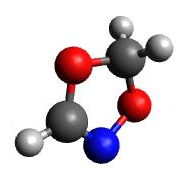
\includegraphics[trim = 0mm 0mm 0mm 0mm, clip,width=0.3\columnwidth]{./figures/Reactant.jpg}
\end{center}
\caption{$C_2O_2H_3N$ molecule.}
\protect{\label{fig:C2O2H3N}}
\end{figure}
The CIPSI method
%\cite{XXXrecentCIPSIpaper}
is implemented in the \textit{Quantum Package} (QP) code\cite{QP} developed by the Caffarel group. Once the trial wavefunction is generated, QP is able to produce output readable by the QMCPACK converter as described in section \ref{sec:convert4qmc}.\\
QP can be installed with multiple plugins for different levels of theory in quantum chemistry. When installing the "QMC" plugin, QP can save the wavefunction in a format readable by the QMCPACK converter. \\

In the following we use the $C_2O_2H_3N$ molecule (Fig \ref{fig:C2O2H3N}) as an example of how to run a multireference calculation with CIPSI as a trial wavefunction for \qmcpack. The choice of this molecule is motivated by its multireference nature. While the molecule remains small enough for CCSD(T) calculations with aug-cc-pVTZ basis set, the D1 diagnostic shows a very high value for  $C_2O_2H_3N$, suggesting a multireference character.  Therefore, an accurate reference for the system is not available and it becomes difficult to trust the quality of a single-determinant wavefunction, even when using the DFT-B3LYP exchange and correlation functional. Therefore, in the following, we show an example of how to systematically improve the nodal surface by increasing the number of determinants in the trial wavefunction.\\

The following steps show how to run from Hartree-Fock to selected CI using QP, convert the wavefunction to a QMCPACK trial wavefunction and finally how to analyze the result.

\begin{itemize}
\item Step 1: Generate the QP input file:\\
QP takes for input an XYZ file containing the geometry of the molecule such as:

\begin{center}
\begin{tabular}{ l c c c }
8\\
C2O2H3N\\
C &       1.067070 &  -0.370798 &   0.020324\\
C &      -1.115770 &  -0.239135 &   0.081860\\
O &      -0.537581 &   1.047619 &  -0.091020\\
N &       0.879629 &   0.882518 &   0.046830\\
H &      -1.525096 &  -0.354103 &   1.092299\\
H &      -1.868807 &  -0.416543 &  -0.683862\\
H &       2.035229 &  -0.841662 &   0.053363\\
O &      -0.025736 &  -1.160835 &  -0.084319   
\end{tabular}
\end{center}

The input file is generated through the following command line:\\

\begin{shade}
qp_create_ezfio_from_xyz C2O2H3N.xyz -b cc-pvtz 
\end{shade}

 
This means that we will be simulating the molecule in all-electrons within the cc-pVTZ basis set. Other options are of course possible such as using ECPs, different spin multiplicities etc. For more details, to the Quantum Package tutorial \url{https://github.com/LCPQ/quantum_package/wiki/Tutorial}.\\
A directory called \textit{C2O2H3N.ezfio} is created and contains all the relevant data to run the SCF Hartree-Fock calculation. Note that due to the large size of molecular orbitals (220), it is preferable to run QP in parallel. QP parallelization is based on a Master/Slave process allowing a master node to manage the work load between multiple MPI processes through the LibZMQ library. In practice one submits the run to one master node, then submits as many nodes as necessary to speed up the calculations. If a "slave" node dies before the end of its task, the master node will resubmit the workload to another available node. If more nodes are added at any time during the simulation, the master node will use them to reduce the time to solution.\\
\item Step 2: Running Hartree-Fock:\\
To save the integrals on disk and avoid recomputing them later, edit the ezfio directory with the following command:\\
\begin{shade}
qp_edit C2O2H3N.ezfio 
\end{shade}

This will generate a temporary file showing all the contents of the simulation and opens an editor to allow modification of their values. Look for \textit{disk\_access\_ao\_integrals} and modify its value from \textit{None} to \textit{Write}\\

To run a simulation with QP, use the binary \textit{qp\_run} with the desired level of theory, in this case Hartree-Fock (SCF). \\
\begin{shade}
mpirun -np 1 qp_run SCF C2O2H3N.ezfio &> C2O2H3N-SCF.out 
\end{shade}

If run in serial, the evaluation of the integrals and the Hamiltonian diagonalization would take a substential amount of computer time. It is recommended to add a few more \textit{slave-nodes} to help speed up the calculation.\\

\begin{shade}
mpirun -np 20 qp_run -slave qp_ao_ints C2O2H3N.ezfio &> C2O2H3N-SCF-Slave.out 
\end{shade}
The total Hartree-Fock energy of the system in cc-pVTZ is \textit{$E_{HF}=-283.0992$}Ha.\\ 
\item Step 2: Freeze Core electrons:\\
In order to avoid making excitation from the core electrons, freeze the core electrons and only do the excitations from the valence electrons.\\  
\begin{shade}
qp_set_frozen_core.py C2O2H3N.ezfio
\end{shade}
This will will automatically freeze the orbitals from 1 to 5, and leave the remaining active. \\
\item Step 3: Atomic orbitals to Molecular Orbital transformation\\
This step, transforming the atomic orbitals to molecular orbitals, is the most costly, especially given that its implementation in Quantum Package is serial. It is recommended to do it in a separate run and on one node.\\
\begin{shade}
qp_run four_idx_transform C2O2H3N.ezfio
\end{shade}

The MO integrals are now saved on disk and unless the orbitals are changed, they will not be recomputed.\\
\item Step 4: CIPSI \\
At this point the wavefunction is ready for the selected CI. By default QP has 2 convergence criteria. The number of determinants (set by default to 1M) or the value of PT2 (set by default to $1.10^{-4}$Ha). For this molecule, the total number of determinants in the FCI space is $2.07e+88$ determinants. While his number is completely out of range of what is possible to compute, we will set the limit of determinants in QP to 5M determinants and see if the nodal surface of the wavefunction is converged enough for the DMC. It is important to remember at this point that the main value of CIPSI compared to other selected CI method, is that the value of PT2 is evaluated directly at each step giving a good estimated of the error to the FCI energy. This allows us to conclude that when the E+PT2 energy is converged, the nodal surface is probably also converged.\\
Similar to the SCF runs, FCI runs have to be submitted in parallel with a \textit{Master/Slave} process:\\

\begin{shade}
mpirun -np 1 qp_run fci_zmq C2O2H3N.ezfio &> C2O2H3N-FCI.out 
mpirun -np 199 qp_run -slave selection_davidson_slave C2O2H3N.ezfio\\
&> C2O2H3N-FCI-Slave.out 
\end{shade}

\item Step 5 (optional): Natural orbitals \\
While this step is optional, it is important to note that using natural orbitals instead of Hartree Fock orbitals will always improve the quality of the wavefunction and improve the quality of the nodal surface by reducing the number of needed determinants for the same accuracy. When a full convergence to the FCI limit is attainable, this step will not lead to any change in the energy but will only reduce the total number of determinants. However, if a full convergence is not possible, this step can increase significantly the accuracy of the calculation at the same number of determinants. \\

\begin{shade}
qp_run save_natorb C2O2H3N.ezfio  
\end{shade}
\hfill

At this point, the orbitals are modified, a new AO$\rightarrow$MO transformation is required and Steps 3 and 4 need to be run again.\\

\item Step 6: Analysis of the CIPSI results\\
\begin{figure}
\begin{center}
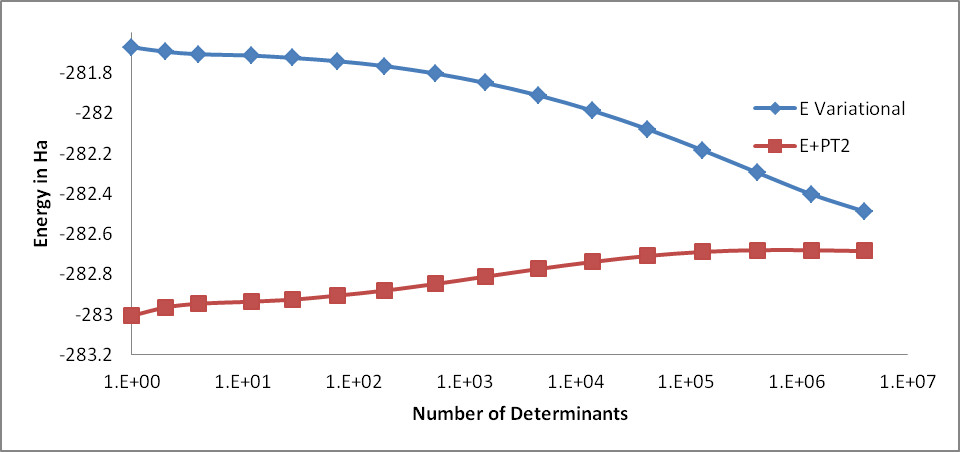
\includegraphics[trim = 2mm 2mm 2mm 2mm, clip,width=0.95\columnwidth]{./figures/CIPSI.jpg}
\end{center}
\caption{Evolution of the variational energy and the Energy + PT2 as a function of the number of determinants for the $C_2O_2H_3N$ molecule.}
\protect{\label{fig:CIPSI}}
\end{figure}
Figure \ref{fig:CIPSI} shows the evolution of the variational energy and the energy corrected with PT2 as a function of the number of determinants up to 4M determinants. While it is clear that the raw variational energy is far from being converged, the Energy + PT2 appears converged around 0.4M determinants.\\



\begin{table}[t]
\centering
\caption{Energies of $C_2O_2H_3N$ using orbitals from Hartree-Fock, natural orbitals, 0.4M and 4M determinants}
\label{TAB:CIPSI}
\begin{tabular}{l|c|c}
\hline \hline
Method & N\_det & Energy\\
\hline
Hartree-Fock &    1    & -281.6729\\
Natural Orbitals & 1 & -281.6735\\
E\_Variational &  438,753 & -282.2951 \\
E\_Variational &  4,068,271   & -282.4882 \\
E+PT2 & 438,753& -282.6809 \\
E+PT2 & 4,068,271 & -282.6805  \\ \hline \hline
\end{tabular}
\end{table}


\item Step 7: Truncation of the number of determinants.\\ While using
  all the 4M determinants from CIPSI always guarantees that all
  important determinants are kept in the wavefunction, practically,
  such a large number of determinants would make any QMC calculation
  prohibitively expensive, as the cost of evaluating a determinant in
  DMC grows as $\sqrt[]{N_{det}}$ where $N_{det}$ is the number of
  determinants in the trial wavefunction. To truncate the number of
  determinants, we follow the method described by Scemama
  \textit{et. al}~\cite{Scemama2018} where the wavefunction is
  truncated by removing independently spin-up and spin-down
  determinants whose contribution to the norm of the wavefunction is
  below a user-defined threshold, $\epsilon$. For this step, we choose
  to truncate the determinants whose coefficients are below,
  $1.10^{-3}$, $1.10^{-4}$, $1.10^{-5}$ and $1.10^{-6}$, translating
  to 239, 44539, 541380 and 908128 determinants, respectively.

To  truncate the determinants in QP, edit the ezfio file as follows:

\begin{shade}
qp_edit C2O2H3N.ezfio  
\end{shade}

then look for \textit{ci\_threshold} and modify the value according to the desired threshold. Use the following run to truncate the determinants:

\begin{shade}
qp_run truncate_wf_spin C2O2H3N.ezfio  
\end{shade}

\item Step 7: Save the wavefunction for \qmcpack \\
The wavefunction in QP is now ready to be converted to \qmcpack format.
Save the wavefunction into \qmcpack format and then convert the wavefunction using the \textit{convert4qmc} tool\\

\begin{shade}
qp_run save_for_qmcpack C2O2H3N.ezfio &> C2O2H3N.dump  
convert4qmc -QP C2O2H3N.dump -addCusp -production
\end{shade}

Since we are running all-electron calculations, orbitals in QMC need
to be corrected for the electron-nuclearcusp condition..  This is done
by adding the option \textit{-addCusp} to \textit{convert4qmc}, which
adds a tag forcing \qmcpack to run the correction or read them from a
file if pre-computed. When running multiple DMC runs with different
truncation thresholds, only the number of determinants is varied and
the orbitals remain unchanged from one calculation to another and the
cusp correction needs only be run once.

\item Step 7: Running \qmcpack \\
At this point, running a multideterminant DMC becomes identical to running a regular DMC with \qmcpack; 
After correcting the orbitals for the cusp, optimize the Jastrow functions and then run the DMC. 
It is however important to mention a few remarks;\\

(1) \qmcpack allows reoptimization of the coefficients of the
determinants during the Jastrow optimization step. While this has
proven to lower the energy significantly when the number of
determinants is below 10k, a large number of determinants from CIPSI
is often too large to optimize conveniently. Keeping the coefficients
of the determinants from CIPSI unoptimized is an alternative strategy.\\

(2) The large determinant expansion and the Jastrows are both trying
to recover the missing correlations from the system. When optimizing
the Jastrows, we recommend to first optimize J1 and J2 without the J3,
and then with the added J3. Trying to initially optimze J1, J2 and J3
at the same time may lead to numerical instabilities.\\

(3) The parameters of the Jastrow function will need to be optimized
for each truncation scheme and usually cannot be reused effeciently
from one truncation scheme to another.

\item Step 8: Analyzing DMC results from \qmcpack \\

From Table \ref{TAB:CIPSI-DMC}, we can see that increasing the number
of determinants from 0.5M to almost 1M determinant keeps the energy
within error bars and does not improve the quality of the nodal
surface. We can conclude that the DMC energy is converged at 0.54M
determinants. It is important to note that this number of determinants
also corresponds to the convergence of E+PT2 in CIPSI calculations,
confirming for this case that the convergence of the nodal surface can
follow the convergence of E+PT2 instead of the more difficult
variational energy.


\begin{table}[t]
\centering
\caption{DMC Energies and CIPSI(E+PT2) of $C_2O_2H_3N$ in function of the number of determinants in the trial wavefunction.}
\label{TAB:CIPSI-DMC}
\begin{tabular}{l|c|c}
\hline 
N\_det & DMC& CISPI\\
\hline
1 & -283.0696 (6)&-283.0063\\
239 & -283.0730 (9)&-282.9063\\
44,539 & -283.078 (1)&-282.7339\\
541,380 & -283.088 (1)&-282.6772\\
908,128& -283.089  (1)&-282.6775\end{tabular}
\end{table}

\end{itemize}

As mentioned in previous sections, DMC is variational relative to the
exact nodal surface. A nodal surface is "better" if it lowers the DMC
energy. To assess the quality of the nodal surface from CIPSI, we
compare these DMC results to other single determinant calculations
from multiple nodal surfaces and theories. Figure \ref{fig:CIPSI-DMC}
shows the energy of the $C_2O_2H_3N$ molecule as a function of
different single-determinant (SD) trial wavefunctions with an
aug-cc-pVTZ basis set, including Hartree-Fock (HF), DFT-PBE and hybrid
functionals B3LYP and PBE0. The last 4 points in the plot show the
systematic improvement of the nodal surface as a function of the
number of determinants. 

When the DMC-CIPSI energy is converged with respect to the number of
determinants, its nodal surface is still lower than the best SD-DMC
(B3LYP) by 6(1)mHa. When compared to CCSD(T) with the same basis set,
$E_{CCSD(T)}$ is 4mHa higher than DMC-CIPSI and 2mHa lower than
DMC-B3LYP. While 6 (1) mHa can seem very small, it is however
important to remember that CCSD(T) cannot describe correctly
multireference systems and therefore it is impossible to assess the
correctness of the SD-DMC result, making CIPSI-DMC calculations an
ideal benchmark tool for multireference systems.

\begin{figure}
\begin{center}
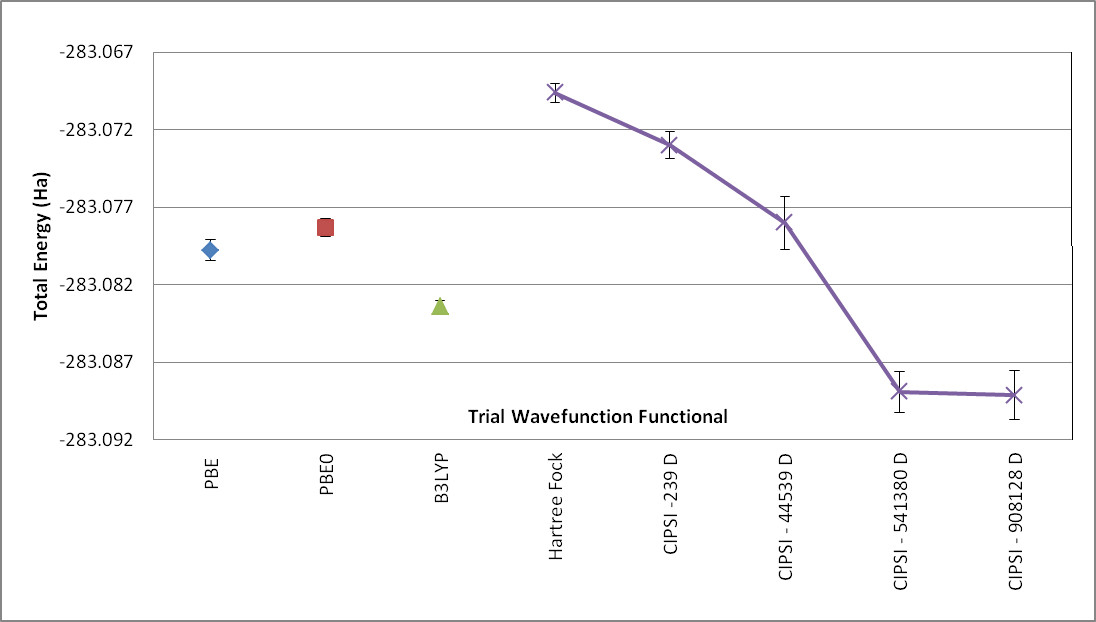
\includegraphics[trim = 2mm 2mm 2mm 2mm, clip,width=0.9
\columnwidth]{./figures/DMC-Multidet.jpg}
\end{center}
\caption{DMC energy of $C_2O_2H_3N$ molecule as a function of different single determinant trial wavefunctions with aug-ccp-VTZ basis set using nodal surfaces from Hartree-Fock (HF), DFT-PBE and DFT with hybrid functionals PBE0 and P3LYP. The CIPSI trial wavefunction contains as indicated 239, 44539, 514380 and 908128 determinants (D). }
\protect{\label{fig:CIPSI-DMC}}

\end{figure}
